% !TeX root = skripta-konstitutivni-vztahy-materialu.tex
% !TeX lastmodified = 2019-12-11

\subsection{Model kinematického zpevnění Chaboche}\label{sec:chaboche}
Pro monotonní jednoosé zatěžování tento model\footnote{Chaboche, J. L., Dang-Van, K. Cordier, G. "Modelization of strain memory effect on the cyclic hardening of 316 stainless steel" In: Transactions of the 5th International Conference on Structural Mechanics in Reactor Technology, Berlin, No. Div L in 11/3, 1979} používá rovnici:
\begin{equation}
	\sigma = \sigma_y + \sum\limits_{i=1}^M \frac{C_i}{\gamma_i} \left[ 1 - \exp\left( -\gamma_i \varepsilon_p \right) \right],
	\qquad
	\varepsilon = \frac{\sigma}{E} + \varepsilon_p
\end{equation}

Pro cyklické zatěžování s~amplitudou napětí $\sigma_a$ a~přetvoření $\varepsilon_a$ má rovnice tvar:
\begin{equation}
	\sigma_a = \sigma_y + \sum\limits_{i=1}^M \frac{C_i}{\gamma_i} \tanh\left( \gamma_i \varepsilon_{ap} \right),
	\qquad
	\varepsilon = \frac{\sigma_a}{E} + \varepsilon_{ap}
\end{equation}
kde
\begin{description}
	\item[$\sigma_y$] je mez kluzu,
	\item[$\varepsilon_p$] je plastické přetvoření,
	\item[$\varepsilon_{ap}$] je amplituda plastického přetvoření,
	\item[$M$] je zvolený stupeň modelu,
	\item[{$C_i\:[\si{\mega\pascal}], \gamma_i\:[-]$}] jsou další parametry modelu.
\end{description}

\begin{figure}[H]
	\centering
	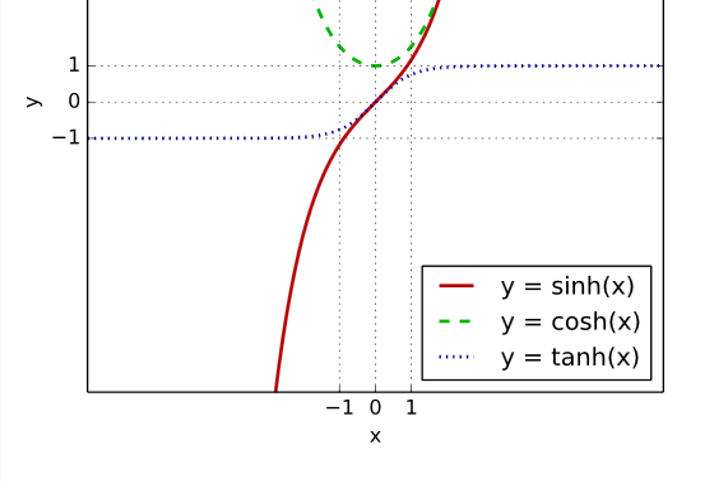
\includegraphics[width=0.7\linewidth]{Obrazky/hyperbolicke-funkce}
	\caption{Průběhy hyperbolických funkcí}
	\label{fig:hyperbolicke-funkce}
\end{figure}
\begin{equation}
	\tanh(x) = \frac{\sinh(x)}{\cosh(x)} = \frac{e^x - e^{-x}}{e^x + e^{-x}} = \frac{1 - e^{-2x}}{1 + e^{-2x}}
\end{equation}

\subsubsection{Kinematické zpevnění při víceosé napjatosti}
Pro víceosou napjatost se posun mezní plochy řídí tenzorovou proměnnou.
\begin{itemize}
	\item A -- prvotní plocha plasticity (bez zpevnění).
	\item B -- následná plocha plasticity se zpevněním v~tahu.
	\item C -- následná plocha plasticity se zpevněním v~tahu a~krutu (prutová napjatost).
\end{itemize}

\begin{figure}[H]
	\centering
	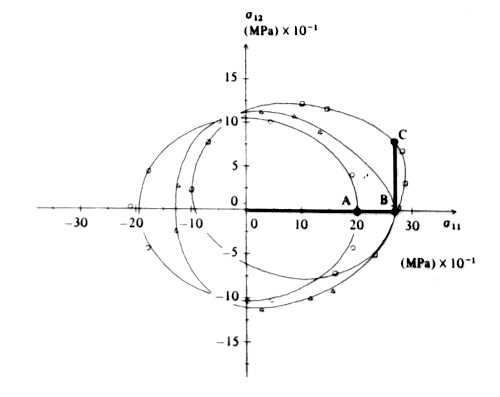
\includegraphics[width=0.7\linewidth]{Obrazky/zavislost-nasledne-mezni-plochy}
	\caption{Závislost následné mezní plochy plasticity na předchozím zatížení v~tahu a~krutu pro hliníkovou slitinu 2024.}
	\label{fig:zavislost-nasledne-mezni-plochy}
\end{figure}

Při víceosé napjatosti dochází ke kombinaci různých typů zpevnění:
\begin{itemize}
	\item izotropní změkčení -- zmenšení následné plochy plasticity,
	\item anizotropní zpevnění -- rotace prvotní plochy plasticity,
	\item kinematické zpevnění -- posun následné plochy plasticity.
\end{itemize}

\begin{figure}[H]
	\centering
	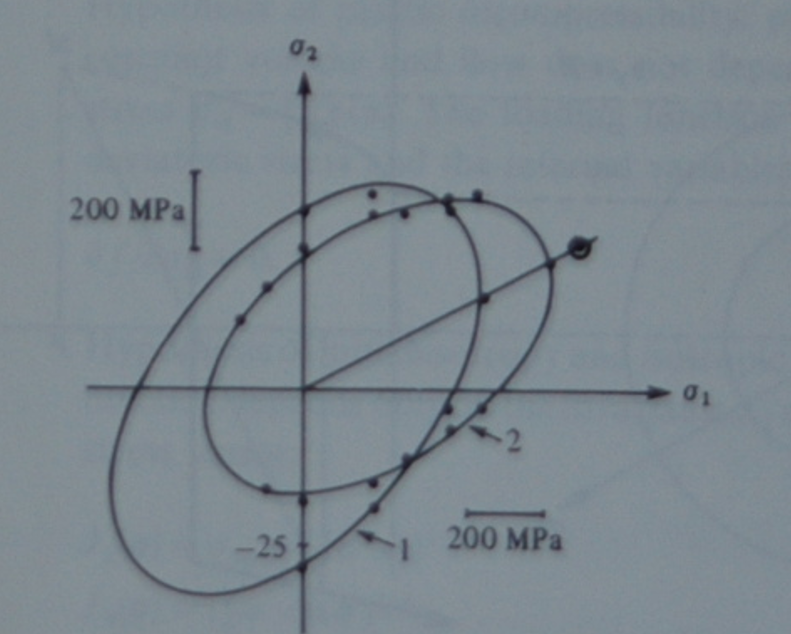
\includegraphics[width=0.7\linewidth]{Obrazky/modifikace-nasledne-mezni-plochy}
	\caption{Modifikace následné mezní plochy plasticity pro ocel 1Cr-1/2Mo-1/4V.}
	\label{fig:modifikace-nasledne-mezni-plochy}
\end{figure}

\begin{figure}[H]
	\centering
%	\includegraphics[width=0.5\linewidth]{}
	\caption{Průběh deformačně-napěťové křivky nad mezí kluzu (jen plastická deformace)}
	\label{fig:deformacne-napetovka-krivka-chaboche}
\end{figure}
